\documentclass{llncs}
\usepackage[ngerman]{babel}
\usepackage[utf8]{inputenc}
\usepackage{listings}
\usepackage{graphicx}

\usepackage{url}
\usepackage{natbib}
\usepackage[autostyle=true,german=quotes]{csquotes}


\title{Hauptprojekt}
\author{Alexander Piehl\\\email{alexander.piehl@haw-hamburg.de}
\institute{Hamburg University of Applied Sciences,\\Dept. Computer Science, \\ Berliner Tor 7\\ 20099 Hamburg, Germany\\}}

\begin{document}
\maketitle
\section{Einleitung}
In der vorliegenden Ausarbeitung wird die erfolgte Arbeit im Hautprojekt vorgestellt. Der Schwerpunkt im Hauptprojekt lag dabei zu prüfen, inwieweit das Framework PACT für eine Microservice Architektur bzw. für das Framework MARS nützlich ist. Mit dem Programm PACT können sogenannte Consumer Driven Contract Tests ausgeführt werden. Bei diesen Tests werden die Schnittstellen zwischen zwei Services getestet, die miteinander interagieren. Der Testansatz Consumer Driven Contract Tests basiert auf de Ansatz Consumer Driven Contract, welcher für die Implementierung von Schnittstellen verwendet werden kann. Bei diesem Ansatz werden die Schnittstellen aus der Sicht des Consumers entwickelt. Dabei ist der Consumer, der Service, der den anderen Service anfragt, also den Request erstellt.

Innerhalb dieser Ausarbeitung soll erarbeitet werden, ob PACT, die im Grundprojekt erarbeiteten Anforderungen für das Testen von Microservice Anwendungen erfüllen kann. Die größten Anforderungen waren dabei, ein schnelles und aussagekräftiges Feedback aus den Tests zu bekommen. Dabei dient weiterhin das Framework MARS als Testobjekt.

Da PACT Schnittstellen testet, wird am Anfang der Ausarbeitung der Architekturstil erläutert, in dem die Schnittstelle von MARS implementiert wurden sind. In MARS sind alle Schnittstellen mit dem Architekturstil REST entworfen worden. Nach der grundsätzlichen Erklärung von REST, werden noch Besonderheiten beim Testen definiert, welche sich aus der Schnittstelle und der Verwendung von REST ergeben. Diese neu ausgearbeiteten Herausforderungen sollen die im Grundprojekt ausgearbeiteten Herausforderungen ergänzen. 
Im nächsten Kapitel wird anschließend Consumer Driven Contract Test detaillierter vorgestellt und erläutert. In diesem Zuge wird die Erläuterung mithilfe einer Beispiel Implementierung von PACT gemacht. Im Anschluss wird im nächsten Kapitel die Implementierung von PACT innerhalb von MARS beschrieben, da sie sich durchaus vom generellen Ablauf unterscheidet. Für die Implementierung von PACT innerhalb von MARS wurden zwei Service ausgesucht, an denen beispielhaft die Implementierung ausgeführt wurden ist. Nach der Implementierung von PACT wurden verschiedene Untersuchungen durchgeführt, die dazu dienten PACT zu bewerten. In dieser Bewertung wird auch eine Aussage getroffen, ob PACT sinnvoll für MARS bzw. generell für eine Microservice Architektur ist. Zum Abschluss dieser Ausarbeitung gibt es noch einen Ausblick auf die Master Arbeit.
\nocite{*}
\section{REST}
REST ist ein Architekturstil für verteilte Systeme. Die Abkürzung REST steht für Representational State Transfer \cite{chakrabarti2009test}.
Erstmals wurde REST im Jahr 2000 von Roy Fielding vorgestellt \citep{kao2013performance}.
Die Rest-Architektur wird häufig für Client-Server Anwendungen verwendet, ist jedoch nicht darauf beschränkt.
Dabei ist REST zurzeit sehr beliebt bei der Entwicklung von Webservices, da aufgrund von REST Webservices wohl nicht nur leichter zu implementieren sind, sondern auch einfacher zu skalieren sind. \cite{chakrabarti2009test}. 
Unter Anderem aus diesen Gründen stellten Google, Facebook und Yahoo ihre Services von SOAP auf REST um \cite{rodriguez2008restful, navas2014rest}.

REST basiert dabei auf Resource Oriented Architecture, kurz ROA \citep{chakrabarti2009test}. Dies bedeutet, dass jede wichtige Information als Ressource zur Verfügung stehen muss \cite{porres2011modeling}.
Die Zugänglichkeit zu der Ressource muss über eine eindeutige URI gegeben sein. Die Ressourcen sollen zusätzlich über verschiedene Methoden manipuliert werden können. Es müssen mindestens die sogenannten CRUD-Operatoren zur Verfügung stehen. CRUD steht für Create, Read, Update und Delete und beschreibt die grundsätzlichen Daten Operationen. Bei Rest werden dafür die standardisierten HTTP-Methoden verwendet, welche im Standard RFC 2616 definiert wurden sind \citep{kao2013performance}. In der Tabelle \ref{tab:CRUD_HTTP_Methods} auf Seite \pageref{tab:CRUD_HTTP_Methods} werden die Beziehung zwischen den CRUD Operatoren und den HTTP Operatoren dargestellt.

\begin{table}[htbp]
\centering
\begin{tabular}{|c|l|p{4cm}|p{4cm}|}
\hline
\multicolumn{1}{|l|}{CRUD-Operation} & HTTP-Methode \\ \hline
Create & POST  \\ \hline
Read & GET \\ \hline
Update & PUT \\ \hline
Delete & DELETE \\ \hline
\end{tabular}
\caption{Beziehung CRUD und HTTP Operatoren \cite{reza2010framework}}
\label{tab:CRUD_HTTP_Methods}
\end{table}

Neben den CRUD-Operatoren können noch weitere HTTP-Methoden zur Verfügung stehen, wie z.B. HEAD und OPTIONS \cite{porres2011modeling}.

Bei REST müssen die jeweiligen Aufrufe Zustandslos erfolgen \cite{reza2010framework, porres2011modeling, kao2013performance}. Im Detail heißt dies, dass der Webservices keine Informationen über den Zustand seiner einzelnen Clients speichert. Sollten Informationen über den Zustand notwendig sein, müssen die Clients die Informationen mitgeben. Dahingehend ist es auch mit REST möglich kompliziertere Programmzustände abzubilden \cite{porres2011modeling}.

Die jeweiligen Nachrichten können in verschiedenen Formate vorliegen
\cite{reza2010framework}. Sehr häufig werden XML oder JSON oder beide Formate für die Nachrichten verwendet. 
Eine Vorschrift existiert nicht.

Zusammenfassend lässt sich REST in vier Grundprinzipien zusammenfassen \citep{porres2011modeling}: 

\begin{itemize}
\item \textbf{Addressability: } Jede wichtige Informationen muss als Ressource vorliegen und über eine eindeutige URI erreichbar sein.
\item \textbf{Connectedness: } Die Repräsentation der Ressourcen ist getrennt von den Ressourcen. Dies bedeutet Ressourcen können in verschiedenen Formate vorliegen, wie JSON und XML.
\item \textbf{Uniform Interface: } Auf die Ressourcen wird nur über standardisierten HTTP-Methoden zugegriffen.
\item \textbf{Statelessnes: } Jede Kommunikation erfolgt Zustandslos.
\end{itemize}

Webservices, welche die vier Grundprinzipien einhalten, bekommen häufig den Beinamen RESTful \citep{porres2011modeling}. Der Begriff RESTful ist jedoch nicht eindeutig definiert.  

Was ist besonders an Rest? Unterschiede zu SOAP? Warum lieber Rest als SOAP?
Leichtgewichtig: leichtes ändern der Schnittstelle möglich

\subsection{Besonderheiten beim Testen ?}
Die Kommunikation zwischen Consumer und Service erfolgt nach einem festgelegten Kontrakt, welcher auch häufig Schnittstelle genannt wird. In dem Kontrakt ist festgelegt, wie die Kommunikation zwischen Consumer und Service aussieht. Das heißt, mit dem Kontrakt ist definiert welche Methoden der Service seinen Consumer anbietet und wie die Consumer sie aufrufen können, also welche Parameter benötigt werden und in welchem Format der Consumer seine Antwort erhält. Dahingehend ist es enorm wichtig, dass der Kontrakt eingehalten wird. Denn ansonsten kann es zu Fehlern führen.

Des Wegen muss ein Schwerpunkt beim Testen von Anwendungen, welche REST verwenden, darauf liegen, zu kontrollieren, dass der Kontrakt weiterhin gültig ist. Daher muss geprüft werden, dass Veränderung am Consumer bzw. Service nicht zur einer Verletzung des Kontraktes führen.

Besonders bei Anwendungen mit einer Microservice-Architektur, bei der die Kommunikation hauptsächlich über das Netzwerk geschieht, ist es von großer Bedeutung, dass die Kommunikation funktioniert und nicht auf Grund fehlerhaften Kontrakten zu Fehlern kommt.

Wegen der Verlagerung der Kommunikation in das Netzwerk, wird das überprüfen der Kontrakte umfangreicher, da schlicht und ergreifend sehr viele Kontrakte vorliegen. Ergänzend dazu sind die einzelnen Services gleichzeitig Consumer und Service Provider. Daher kann es schnell unübersichtlich werden, wer welchen Services anfragt und wie.

Besonders bei gewünschten Änderungen eines Kontraktes kann es unübersichtlich werden. Aufgrund der möglichen Vielzahl von Consumer, kann  sehr schnell der Überblick verloren werden, welche Consumer aktualisiert werden müssen und welche nicht. Dies kann zur Folge haben, dass ein Service Methoden oder Variante einer Methode bereitstellt, die nicht mehr benötigt werden.

Eine andere Problematik, die durch der Verlagerung der Kommunikation in das Netzwerk, entsteht ist, dass sehr viel Traffic im Netzwerk herrschen kann. Dadurch kann es vermehrt auftreten, dass Nachrichten beschädigt werden oder auch verloren gehen. Mit dieser Problematik müssen die Services und Consumer umgehen können.

\section{Consumer Driven Contract Test}
Bei dem Ansatz Consumer-Driven Contracts werden die Schnittstellen bzw. die Verträge aus der Sicht des Clients/Consumers definiert \cite{Robinson2006}. Dabei spielt es keine Rolle, ob es nur einen Cosumer oder mehrere existieren. Die jeweiligen Anfragen und gewünschten Antworten werden notiert und auf Grundlage dieser Informationen wird der Service implementiert. Dabei baut der Ansatz auf der Grundnahme auf, dass der Consumer am besten wüsste, was er nutzen möchte.

Wie sich aus der generellen Beschreibung dieses Ansatzes ableiten lässt, eignet sich dieser Ansatz am Besten, wenn sowohl die Consumer wie der Service neu implementiert werden. Bei bestehenden Anwendungen könnte dieses Verfahren unter anderem dafür genutzt werden, um zu überprüfen, ob der Service unnötige Schnittstellen bzw. Methoden anbietet.

Der Ansatz Consumer Driven Contract hat den Vorteil, dass sehr klar definiert ist, welche Anforderungen der Consumer bzw. die Consumer an den Services haben. Andernfalls könnte der Service nur erahnen, wie er die jeweiligen Anfoderungen umsetzen muss. Durch die eindeutige Definierung der Anforderungen, kann der Service so schlank wie möglich implementiert werden.   

Auf der Basis dieses Konzeptes setzen die Consumer Driven Contract Tests auf. Ein Tool, welches Consumer Driven Contract Tests unterstützt ist PACT. PACT ist ein Open-Source Tool, welches auf Github verwaltet wird.

In der Ausführung von Toby Clemson über das Testen von Microservices wird dieses Verfahren explizit empfohlen. Dabei benennt er neben PACT noch zwei weitere Tools, welche Consumer Driven Contract Tests anbieten. Diese Tools sind PACTO und Janus. Für das Hauptprojekt wurde sich für PACT entschieden, da nach der ersten Recherche PACT den größten Umfang bietet und zudem PACT besser dokumentiert ist, als die anderen Tools.

Mit dem Tool PACT können die Consumer Driven Contract Tests in verschiedenen Programmiersprachen geschrieben werden. Zur Auswahl stehen dabei Ruby, C\#, JavaScript und Java. Im nächsten Kapitel wird der generelle Ablauf von PACT anhand eines Beispiels erläutert, bevor im darauffolgenden Kapitel die Vorteile beschrieben, die durch die Verwendung von Consumer Driven Contract Tests entstehen sollen. Denn einige vermeintliche Vorteile leiten sich direkt aus dem Ablauf von Consumer Driven Contract Test ab.

\subsection{Ablauf Consumer Driven Contract Test}
In diesem Kapitel wird der generelle Ablauf von Consumer Driven Contract Tests beschrieben. Der Ablauf wird anhand mehrere Beispiele erläutert, welche von verschiedenen Seiten stammen, die Consumer Driven Contract Tests erläutern \cite{bayer2015jaxcenter, vitz2016inno, Vincent2015}.

Wie bereits erläutert basiert Consumer Driven Contract Test auf Consumer Driven Contract. Daher wird auch bei Consumer Driven Contract Test zunächst der Consumer bzw. die Consumer implementiert. In diesem, Beispiel fragt der Consumer Produktdetails über ein bestimmtes Produkt beim Provider an.

Nach dem die Implementierung des Consumers soweit erfolgt ist, dass er Anfragen stellen und verarbeiten kann, kann PACT für den Consumer implementiert werden. Der größte Aufwand bei PACT ist die Implementierung der Testfälle auf der Seite des Consumers.

Für die Implementierung von PACT auf der Seite vom Consumer wird eine neue Klasse angelegt. Diese Klasse erbt von der PACT Klasse ConsumerPactTest. Durch die Vererbung müssen vier abstrakte Methoden implementiert werden, welche in der folgenden Auflistung genannt werden:
\begin{itemize}
\item providerName
\item consumerName
\item createFragment
\item runTest
\end{itemize}


Mit den Methoden providerName() und consumerName() werden die jeweiligen Bezeichnungen als String zurückgegeben. Der Hintergrund dafür ist, dass man damit mehrere PACT Tests für unterschiedliche Provider und Consumer definieren kann.
\lstset{language = Java}
\begin{lstlisting}
    @Override
    protected String providerName() {
        return "Product_Details_Service";
    }

    @Override
    protected String consumerName() {
        return "Product_Service";
    }
\end{lstlisting}

Über die Methode createFragment werden wie Aufrufe des Consumers mit den zu erwartetenden Antworten erstellt. Dies geschieht mit einer von PACT definierten DSL.
\lstset{language = Java}
\begin{lstlisting}
    @Override
    protected PactFragment createFragment(PactDslWithProvider builder) {
        Map<String, String> headers = new HashMap<>();
        headers.put("Content-Type", "application/json;charset=UTF-8");
        
        return builder
        		.uponReceiving("a request for product details")
                .path("/productdetails/1")
                .method("GET")
                .willRespondWith()
                .headers(headers)
                .status(200)
                .body("{\"id\":1,\"description\":\"Thisis the description for product 1\"}")
                .toFragment();
    }
\end{lstlisting}
Zunächst wird eine Map erstellt, in der verschiedene Optionen für den Header definiert werden können. In diesem Fall wird nur der  Content-Type auf JSON mit dem Zeichensatz UTF-8 festgelegt. Als Rückgabewerttyp gibt die Methode ein sogenanntes PactFragment zurück. Diese PactFragment wird vom PactDslWithProvider erstellt, welches der Methode als Parameter übergeben wird. Da damit das Fragment erstellt, bekommt es den passenden Namen builder. Mit des Builder können die verschiedenen Interaktionen definiert werden.


\begin{itemize}
\item \textbf{uponReciving: } Mit dieser Metohde wird eine neue Interaktion erstellt. Als Parameter bekommt sie eine Beschreibung der Interaktion.
\item \textbf{path: } Der Methode path wird der aufzurufende Pfad als Parameter übergeben.
\item \textbf{method: } Über die Methode method wird festgelegt mit welcher HTTP-Methode der Aufruf erfolgt.
\item \textbf{willRespondWith: } Die Methode gibt an, dass ab hier die zu erwartetende Antwort definiert wird.
\item \textbf{headers: } Über dieser Methode kann definiert werden, dass entsprechende Werte im Header vorhanden sein müssen.
\item \textbf{status: } Soll der Statuscode überprüft werden, kann mit dieser Methode der zu erwartetende Statuscode definiert werden.
\item \textbf{body: } Mit der body wird definiert, welcher Body in der Response erwartet wird.
\item \textbf{toFragment: } Zum Abschluss wird die Methode toFragment aufgerufen, mit der das Fragment abgeschlossen wird.
\end{itemize}

Es können auch mehrere Interaktionen mithilfe des Builders erstellt werden. Jeder Interaktion beginnt mit der uponReciving. Um eine weitere Interaktion hinzufügen, kann man einfach nach der Definition der zu erwartetenden Antwort einfach mit der Methode uponReciving eine neue Interaktion hinzugefügt werden, welche nach dem gleichem Schema abläuft. In diesem Beispiel wäre dies nach der Methode body.

Sobald das PactFragment, welches die Interaktionen enthält, implementiert ist, kann getestet werden, ob der Consumer selber den Kontrakt einhält. Dafür wird die Methode runTest umgesetzt.

\lstset{language = Java}
\begin{lstlisting}
@Override
protected void runTest(String url) {
    URI productDetailsUri = URI.create(String.format("%s/%s/%s", url, "productdetails", 1));

    ProductDetailsFetcher productDetailsFetcher = new ProductDetailsFetcher();
    ProductDetails productDetails =  productDetailsFetcher.fetchDetails(productDetailsUri);
    assertEquals(productDetails.getId(), 1);
}
\end{lstlisting}

PACT erstellt auf Grundlage des PactFragments einen Stub vom Provider. Die passende URL zum Provider Stub wird der Methode runTest via Parameter übergeben. Einerseits wird getestet, ob der Consumer eine korrekte Anfrage erstellt und anderseits , ob der Consumer mit der Antwort vom Provider Stub zurecht kommt. Dies wird unter anderem mithilfe von asserts gelöst.

Sobald alle Methoden korrekt implementiert wurden sind, kann die Klasse ausgeführt werden. Entweder kann die Klasse direkt gestartet werden oder man führt die Tests mithilfe eines Maven/Gradle-Plugins von PACT aus.

Sind die Tests erfolgreich durchgelaufen, wird automatisch das sogenannte PACT-File erstellt.

\lstset{language = Java}
\begin{lstlisting}
{
  "provider" : {
    "name" : "Product_Details_Service"
  },
  "consumer" : {
    "name" : "Product_Service"
  },
  "interactions" : [ {
    "description" : "a request for product details",
    "request" : {
      "method" : "GET",
      "path" : "/productdetails/1"
    },
    "response" : {
      "status" : 200,
      "headers" : {
        "Content-Type" : "application/json;charset=UTF-8"
      },
      "body" : {
        "id" : 1,
        "description" : "This is the description for product 1"
      }
    }
  } ],
  "metadata" : {
    "pact-specification" : {
      "version" : "2.0.0"
    },
    "pact-jvm" : {
      "version" : "2.1.7"
    }
  }
}
\end{lstlisting}

Das PACT-File ist im Prinzip eine Zusammenfassung der zuvor definierten Klasse. Es befinden sich die jeweiligen Provider und Consumer Namen drin sowie die definierten Interaktionen und die zu erwarteteden Antworten. Ergänzend dazu ist im PACT-File noch angegeben mit welchen Versionen, die Datei erstellt worden ist.

Mit dem eben nun erstellten PACT-File kann der Provider gestestet werden. Dafür muss der Provider entweder das Gradle oder Maven Plugin von PACT für den Provider verwenden. Um das Plugin verwenden zu können, muss einmal der Pfad zum PACT-File angegeben werden. Das PACT-File kann lokal vorliegen, es kann aber auch via eine URL aufgerufen werden. Zusätzlich muss die Adresse des Providers angegeben werden. Die entsprechenden Einstellungen am Beispiel der Verwendung von Gradle sieht so aus:

\lstset{language = Java}
\begin{lstlisting}
pact {
    serviceProviders {
    productDetailsServiceProvider {
        protocol = 'http'
        host = 'localhost'
        port = 10100
        path = '/'
        hasPactWith('productServiceConsumer') {
            pactFile = file("../product-service/target/pacts/Product_Service-Product_Details_Service.json")
			}
		}
	}
}
\end{lstlisting}

Damit der Test ausgeführt werden kann, muss der Provider gestartet werden. Sobald dies geschehen ist, kann das Plugin für den Provider ausgeführt werden. Das Ergebnis des Tests werden in dann in der Konsole angezeigt.

\begin{itemize}
\item Implementierung Consumer
\item Definieren der Aufrufe
\item PACT für Consumer vorbereiten
\begin{itemize}
\item createFragment
\item providerName
\item consumerName
\item runTest
\end{itemize}
\item erstelltes PACT-File
\item Verfiy mit Maven Plugin des Providers
\item weiteres Vorgehen
\end{itemize}


\subsection{Vorteile Consumer Driven Contract Test}
Neben den generellen Vorteilen, welche man sich von dem Ansatz Consumer Driven Contract Test verspricht und schon im vorherigen Kapitel kurz skizziert wurden sind, gibt es noch weitere Vorteile, die sich explizit auf das Testen beziehen.

In der vorherigen Ausarbeitung zum Grundprojekt wurden die Anforderungen beschrieben, welche beim Testen einer Microserive Anwendung vorliegen. 
Eine dieser Anforderung war, dass das es vom Testen ein schnelles Feedback gibt. 
Genau diese Anforderung soll Consumer Driven Contract Test erfüllen. 
Jede noch so große Änderung am Service soll ohne großen Aufwand gegen das PACT-File getestet werden können. Dadurch soll man eine schnelles Feedback bekommen, ob der Service den Vertrag noch einhält.

Ergänzend dazu verspricht Consumer Driven Contract Test einen feinkörnigen Einblick darin, was die Änderung am Service für Auswirkung hat.

Dazu soll man schnell ein Überblick bekommen, ob die Änderung am Service zu unerwarteten Fehlern führt. Aufgrund des zügigen Feedbacks könnte das Fehlverhalten schnell korrigiert werden.

Bei gewünschten oder notwendigen Änderungen am Service, weil ein neuer Consumer hinzugefügt wurden ist oder es sich bei einem Consumer die Anforderungen an den Service geändert haben. soll man aufgrund von Consumer Driven Contract Test schnell erkennen, ob aufgrund der Änderung andere Consumer angepasst werden müssen. 

Zusammenfassend betrachtet lassen sich die vermeintliche Vorteile von Consumer Driven Contract Test dahingehend vereinen, dass es ein schnelles Feedback gibt, welche Auswirkung die Änderung am Service auf den Kontrakt hat. Dadurch können ungewollte Fehler schnell identifiziert werden oder notwendige Aktualisierungen von Consumer festgestellt werden.

Für ein System wie MARS mit einer Microservice-Architektur bei der das Messaging im Netzwerk extrem relevant ist, sind Fehler aufgrund von falschen Schnittstellen und/oder falschen Anfragen sehr kritisch. Dazu ändern sich innerhalb von MARS immer wieder die Anforderungen, an die auch die jeweiligen Services angepasst werden müssen. Aufgrund der Architektur besteht die Möglichkeit Änderungen schnell umzusetzen und den Service zu deployen. Consumer Driven Contract Test ist dabei sehr vielversprechend diesen Prozess zu begleiten, da es schnelles Feedback geben soll, welche Auswirkungen die Änderungen haben. Ob Consumer Diven Contract Test die beschriebenen Vorteile einhält, wird im nächsten Abschnitt behandelt, bei dem es um die Umsetzung von Consumer Driven Contract Test innerhalb von MARS geht.

\begin{itemize}
\item Vorteile bei Änderungen im Service kann sofort wieder gegen die Datei getestet werden, um zu prüfen, ob alle Consumer noch korrekt funktionieren
\item übersicht, was die Consumer Anfragen
\item sachnelles Feedback
\item wissen, ob Änderung zu ungewollten Fehlern
\item wissen, welche consumer aktualisiert werden müssen
\item MARS System, welches regelmäßig angepoasst wird
\item Architektur, welche Fokus auf des Netzwerk hat
\item Fehler wegen Schnittstelle problematisch
\end{itemize}
Was verspricht man sich davon?
Verbindung zu MARS - System im Wandel

\begin{itemize}
\item Erklärung Consumer Driven Ansatz
\begin{itemize}

\item Vorteile dazu gibt es einen feinjörnigen Einblick und schnelles Feedback für das planen von Änderungen. Ergänzend dazu können gezielt einzelnen Consumer angesprochen werden.
\end{itemize}
\item Erläuterung Consumer Driven Contract Test
\begin{itemize}
\item Tool PACT
\item Consumer definiert seine Anfrage und die zu erwarteten Antworten, samit UNIT-Test
\item Implmentierung im Consumer
\item Beim Ausführen dieser Tests wird ein Server gestartet, der mit den entsprechenden Antworten auf die Anfragen reagiert
\item Dabei wird ein File erstellt, welches die Aufrufe und Antworten enthält
\item mit diesem File wird nun der Service Provider getestet
\item Antwortet er auf die Anfragen korrekt, wie es im File beschrieben ist

\end{itemize}
\end{itemize}


\section{Consumer Driven Contract in MARS}
Nach der grundlegenden Befassung mit PACT soll nun geprüft werden, ob sich PACT für MARS anbietet. Wie schon im Kapitel zu den vermeintlichen Vorteilen von PACT beschrieben, könnte PACT einige Anforderungen an die Tests zu erfüllen. Kurz zusammen gefasst geht es um ein schnelles Feedback der Tests, besonders bei Änderungen am Source Code sowie eine demtentsprechendes aussagekräftiges Feedback.

Im Gegensatz zum eigentlichen gedachten Ablauf von PACT ist MARS ein sehr fortgeschrittenes System, was kurz vor den ersten Release steht. Dies hat zur Folge das PACT in ein bestehendes System eingebunden werden muss und nicht gleichzeitig mit der Implementierung des Consumers bzw. Providers mit eingeführt werden kann.

Ergänzend dazu ist MARS ein sehr umfangreiches System mit vielen verschiedenen Consumern und Providern. Dahher wird PACT zunächst nur in einem übersichtlichen Teil von MARS verwendet, um eine Machtbarkeitsstudie zu erstellen, ob die Verwendung von PACT innerhalb von MARS sinnvoll ist.

Für die Erstellung der Machtbarkeitsstudie wurde der Bereich der Imports in MARS ausgewählt. Für diese Entscheidung sprechen mehrere Gründe. Zum einem ist es für eine Microservice Architektur ein relatives geschlossenes System und zum anderem sind die einzelnen Komponenten übersichtlich. Dazu ist man in der Lage diesen Bereich des Systems schnell mit Testen zu befüllen. Für die exakte Implementierung von PACT werden die Interaktionen zwischen dem Metadata-Client (Consumer) und dem Provider Metadata verwendet.

\begin{figure}[htbp]
  \centering
      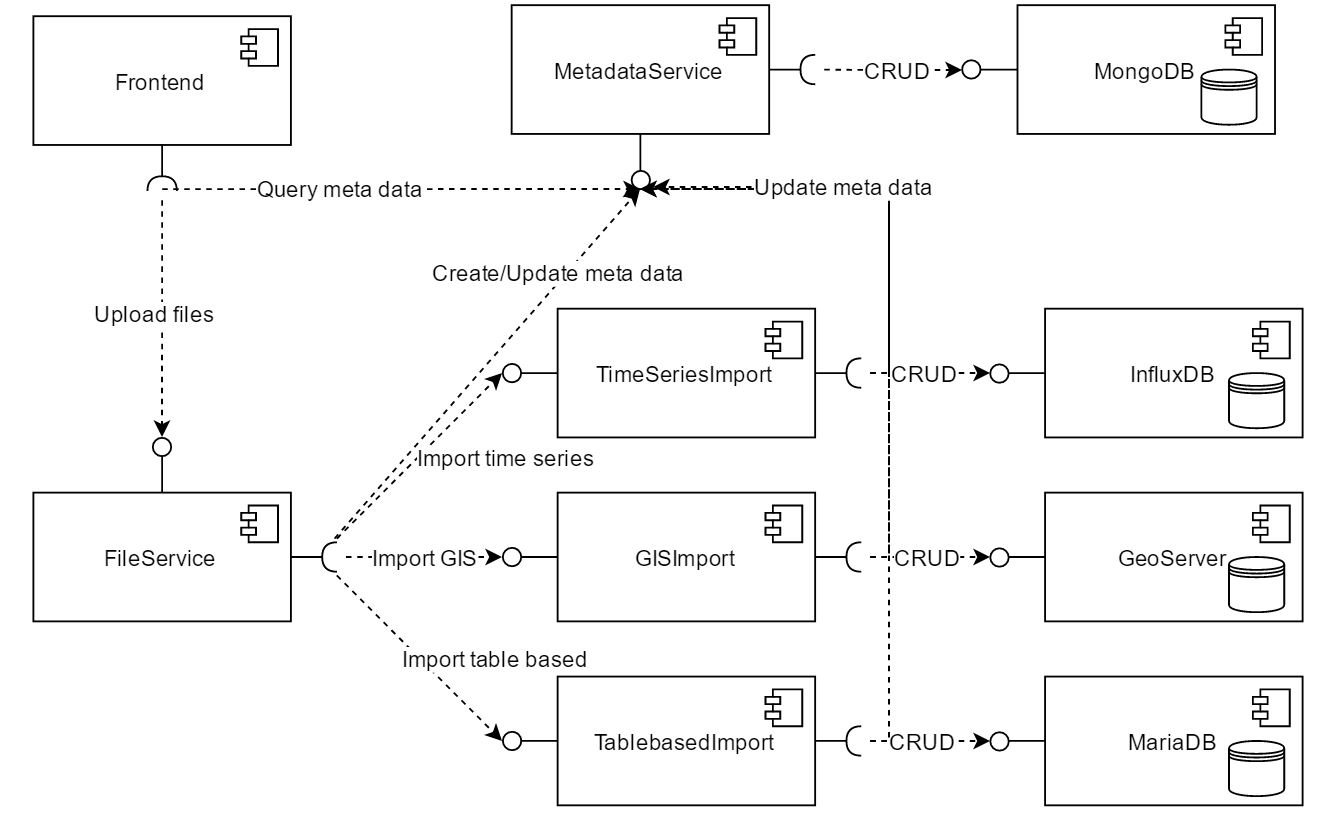
\includegraphics[width=1\textwidth]{./Images/ImportServices}
    \caption{Diagramm der Komponenten für die Import Services}
    \label{fig:ImportServices}
\end{figure}

Wie in der Abbildung \ref{fig:ImportServices} zu den Import Services gut erkenntlich interagieren alle Services, die für den Import zuständig sind, mit dem Service Metadata. Der Service Metadata hat die Aufgaben für die einzelne Dateien, die importiert werden, Metadata zu erstellen, zu aktualisieren und ggf. zu löschen. Die erstellten Metadata werden dann in einer Datenbank abgelegt. Dazu kann das Frontend via des Services Metadata auf die einzelnen Metadata zugreifen. Damit nicht jeder Service, der mit dem Service Metadata interagiert die Aufrufe selber implementieren muss und damit ggf. Redundanzen erzeugt, ist die Kommunikation mit dem Service Metadata im Objekt Metadata-Client gekapselt. Wenn eine Interaktion mit dem Service Metadata erforderlich ist, wird das Objekt Metadata-Client erzeugt, welches dann die Interaktionen übernimmt.

\subsection{Testumgebung}
Die verwendete Testumgebung ist sehr ähnlich zu der Testumgebung im Grundprojekt. Jedoch wurde nicht mehr mit einer virtuellen Maschine gearbeitet, da der VM nicht genug Leistung zugeteilt werden konnte. Daher wurde Linux Ubuntu als Host-System verwendet. Dies bedeutet aber auch, dass kein geschlossenes System mehr für das Testen verwendet wurde. 

Zudem wurde wieder Docker in Verbindung mit dem Tool Docker-Compose verwendet, da das Ausführen von MARS ohne Docker nicht möglich ist. Die Installation von MARS erfolgte nach der gleichen Vorgehensweise, wie im Grundprojekt. 

Ähnlich wie im Grundprojekt wurde auf einem GIT Branch gearbeitet und zwar wurde von den Import-Projekten ein Branch erstellt. Zum Zeitpunkt der Untersuchung von PACT innerhalb von MARS, gab es laufend Änderungen an den Services für den Import. Dies betraff teilweise auch die Schnittstelle. Um sich ausschließlich auf die Einbindung von PACT zu konzentrieren, wurde der Brach erstellt, damit keine Änderungen diesen Prozess beeinträchtigen können.

Für die Implementierung von PACT wurde Intellij als Entwicklungsumgebung verwendet. Dazu wurde Maven als Build-Management-Tool verwendet, da alle MARS-Projekte Maven verwenden und eine Umstellung auf Gradle zu viel Ressourcen verbraucht hätten, ohne vornhinein ermitteln zu können, ob es sich dadurch Vorteile ergeben. Ergänzend dazu wurden die Entwicklungswerkzeuge von Chromium und das Programm Postman verwendet, um die Interaktionen besser zu verstehen und MARS mit default Werten zu füllen. Zusätzlich wurde ein Framework für die Erstellung von Mocks verwendet und zwar das Framework Mockito.

\subsection{Einbindung in MARS}
Zwischen dem Metadata-Client und Metadata gibt es mehrere verschiedene Interaktionen. Dabei sind alle CRDU-Methoden, also GET,POST,PUT und DELETE, vertreten. Bei der Implementierung von PACT wurden jedoch nicht alle Interaktionen umgesetzt, da es zu aufwendig gewesen wäre. In der Tabelle \ref{tab:Interaktionen_PACT} auf der Seite \pageref{tab:Interaktionen_PACT} sind die Interaktionen kurz beschrieben, welche mit PACT implementiert werden sollten.

\begin{table}[htbp]
\centering
\begin{tabular}{|c|l|p{4cm}|p{4cm}|}
\hline
\multicolumn{1}{|l|}{Methode} & Beschreibung \\ \hline
GET & Bekomme einen Metadata-Eintrag via der spezifischen DataID zurück\\ \hline
GET & Bekomme alle Metadata-Einträge zurück \\ \hline
PUT & Aktualisiere die Variable, die den aktuellen Zustand des Uploads beschreibt \\ \hline
POST & Erstelle einen neuen Metadata-Eintrag \\ \hline
DELETE & Lösche einen Metadata-Eintrag via DataID\\ \hline
\end{tabular}
\caption{Interaktionen, die mit PACT umgesetzt wurden sind}
\label{tab:Interaktionen_PACT}
\end{table}

Als Soll-Zusand für die Tests wurden der Zustand genommen, der bei der Erstellung des Branches vorlag. Mithilfe dieses Soll-Zustandes wurden die Interaktionen in PACT implementiert. Als vorbereitetet Schritt davor, mussten die Interaktionen genauer analysiert werden, damit klar definiert werden kann, wie die Anfrage und die dazu gehörige Antwort auszusehen hat.

Bei MARS werden die APIs mithilfe von Swagger\citep{swagger} dokumentiert. Swagger ist ein open source Franework, welches beim Entwerfen, bei der Erstellung und Dokumentation unterstützen soll. Swagger erstellt für jede API eine extra Datei, in welcher die Schnittstellen beschrieben werden. Die Datei heoßt mesitens swagger.yaml. An der Endung der Datei kann man erkennen, dass es sich die Datei im YAML-Format vorliegt. In dieser Datei sind alle Methoden beschrieben, die vom Consumer angefragt werden können. Zu den einzelnen Methoden sind wichtige Infromationen angegeben, wie z.B. der Pfad, die Paramter, die erwartet werden. Zu den Parameter ist noch angegeben, welcher Typ vorliegen soll und wie sie mit geschickt werden sollen, also ob sie z.B. im Body als Query im Pfad mitgeschickt werden sollen. Die Swagger-Datei ist sehr hilfreich für das Programm Postman.

Postman ist ein Programm, welches ähnlich wie Swagger bei der Entwicklung und Dokumentation von Schnittstellen ünterstützen sollen. Bei Postman liegt der Fokus aber auf dem Testen von Schnittstellen und außerdem fügt es im Gegensatz zu Swagger über eine grafische Oberfläche. Mit Postman können Anfragen an einen Provider gestellt werden, um im Anschluss die Antwort zu überprüfen. 

Die mit Swagger erstellte Datei kann in Postman importiert werden und Postman erstellt auf Grundlage der Informationen aus der Swagger-Datei automatisch Testfälle. Jedoch fehlt diesen Testfällen Bedingungen, ob sie erfolgreich sind. Diese Bedingungen können mit einer von Postman definierten DSL selbst implementiert werden. Postman bietet dafür Templates, um standardmäßige Überprüfungen auf Statuss Code oder ähnliches schnell umsetzen zu können.

Da leider manche Informationen in der Swagger-Datei fehlten oder veraltet waren, mussten die automatische Tests manuell aktualisiert werden. Dafür waren die Entwicklungswerkzeuge vom Browser Chromium bzw. Chrome sehr hilfreich. Denn die einzelnen Interaktionen können einem Tool aufgezeichnet und analysiert werden. Dafür wurden die jeweiligen Interaktionen über das Frontend aufgezeichnet und anschließend ausgewertet. Mithilfe dieser Informationen wurden die Testfälle innerhalb von Postman aktualisiert. Sobald alle Tests in Postman implementiert wurden sind und erfolgreich abliefen, wurde damit begonnen PACT auf der Seite des Consumers einzubinden. Jedoch gab es ein Problem mit der DELETE-Methode. Beim Testen mit Postman konnte der Aufruf nicht ausgeführt werden. Der Service antworte mit dem Statuscode 405. Dies bedeutet, dass die gewählte Methode nicht erlaubt ist. Die Methode wurde jedoch in PACT implementiert, da es sich um einen Bug handelt. Dahingehend wurde die Implementierung der DELETE-Methode in PACT alleine auf Grundlage der Swagger-Datei ausgeführt.

\subsubsection{Implementierung des Consumers}
Bei der Implementierung von PACT beim Consumer wurde so ähnlich vorgegangen, wie im allgemeinen Beispiel beschrieben. Auch hier wurde zunächst eine neue Klasse erstellt und zwar die Klasse MetadataClientConsumerTest, welche von ConsumerPactTest erbt. Damit waren wieder die vier Methoden providerName, consumerName, createFragment und runTest vorgegeben. Der Consumer bekam den Namen metadata-client und der Provider den Namen metadata-service. 

In den Methoden createFragment und runTest sind jeweils alle fünf Interaktionen angebildet. Aus Gründen der Übersichtlichkeit wird die Umsetzung einer Interaktionen nach der anderen Interaktionen beschrieben.

Begonnen wurde mit der Interaktionen, bei der via GET ein spezifischer Metadata Eintrag abgefragt werden soll.
Der für diese Interaktion spezifische Code-Abschnitt in der Methode createFragment ist in \ref{lst:getCreateFragment} abgebildet.

\lstset{language = Java}
\begin{lstlisting}[caption=Test,label=lst:getCreateFragment]
.uponReceiving("Get a metadata entry")
.path("/metadata/" + dataID)
.method("GET")
.headers(headerReq)
.query("")
.body("")
.willRespondWith()
.headers(headersRes)
.status(200)
.body(createJsonBody())
\end{lstlisting}

Wie in der Erklärung von REST erwähnt, muss jede Ressource über eine eindeutige URI erreicht werden. Bei den Metadata Einträgen erfolgt dies über die Eigenschaft DataID. Daher wird dem Pfad einfacher der Wert DataID angehängt. Weitere Informationen sind in der Query und Body nicht notwendig. Im Header ist nur definiert wurden, dass nur JSON akzeptiert wird.
Der Provider soll auf diesen Aufruf mit dem Statuscode 200 antworten. Obwohl ein Header für die Antwort definiert ist, findet keine Überprüfung statt, da der Header keine Werte enthält. 

Bis auf die einzelnen Werte unterscheidet sich dieses Fragment nicht vom generellen Beispiel. Nur der Body, welcher die Antwort enthalten soll, ist deutlich umfangreicher. Dafür wird beim Body die Methode createJsonBody aufgerufen, die die zu erwartendete Antwort im Body definiert. Diese Methode ist abgebildet in \ref{lst:createJsonBody}. Ähnlich wie bei der Erstellung des Fragments wird auch für die Erstellung des Body eine PACT definierte DSL genutzt.

\lstset{language = Java}
\begin{lstlisting}[caption=Test,label={lst:createJsonBody}]
private PactDslJsonBody createJsonBody() {
    PactDslJsonBody body = new PactDslJsonBody()
        .stringValue("dataId",dataID)
        .stringType("title")
        .stringType("description")
        .integerType("projectId")
        .integerType("userId")
        .stringValue("privacy","PRIVATE")
        .stringValue("state","FINISHED")
        .stringValue("errorMessage",null)
        .stringValue("records",null)
        .stringValue("type",null)
        .stringValue("geoindex",null)
        .object("additionalTypeSpecificData")
            .object("topLeftBound")
                .decimalType("lng")
                .decimalType("lat")
            .closeObject()
            .object("bottomRightBound")
                .decimalType("lng")
                .decimalType("lat")
            .closeObject()
        .closeObject()
        .asBody();
    return body;
}
\end{lstlisting}

Wie man aus \ref{lst:createJsonBody} gut ableiten kann, ist das Metadata-Objekt recht umfangreich. Da bei der Anfrage definiert wurde, dass nur JSON akzeptiert wird, muss die Antwort selbstverständlich im JSON-Format vorliegen. Um komplexere Antworten in JSON zu definieren, bietet PACT unter anderem die Klasse PactDslJsonBody an. Damit kann ein Objekt erstellt werden, welches unterschiedliche Eigenschaften haben kann. Die einzelnen Methoden fügen nicht nur die Eigenschaften hinzu, sondern definieren auch die jeweiligen Matcher mit. Generell wird der Typ der jeweiligen Eigenschaften bestimmt und sollte kein Wert angegeben werden, wird ein zufälliger Wert vom festgelegten Typ erstellt. Dazu muss immer der Name der jeweiligen Eigenschaft mitangegeben werden. Die bei der Erstellung des JSON-Bodys verwendeten Methoden sind in der Tabelle \ref{tab:Methoden_jsonBody} auf Seite \pageref{tab:Methoden_jsonBody} näher beschrieben.

\begin{table}[htbp]
\centering
\begin{tabular}{|c|l|p{4cm}|p{4cm}|}
\hline
\multicolumn{1}{|l|}{Methode} & Beschreibung \\ \hline
stringValue & Name, Typ Wert müssen übereinstimmen. \\ \hline
stringType & Name und Typ müssen übereinstimmen. \\ \hline
intergerType & Name und Typ müssen übereinstimmen. \\ \hline
decimalType & Name und Typ müssen übereinstimmen. \\ \hline
object & Erzeugung eines Objektes. Name muss übereinstimmen  \\ \hline
closeObject & Schließen des Objektes\\ \hline
asBody & Abschließende Methode, um es in den Typ PactDslJsonBody zu casten. \\ \hline
\end{tabular}
\caption{Erklärung der verwendeten PACT DSL Methoden}
\label{tab:Methoden_jsonBody}
\end{table}

Der damit definierte Body soll die in abgebildete Antwort darstellen. Werte werden nur überprüft, wenn sie aufgrund der Anfrage sicher vorliegen sollte. Wenn die Metadata von einer entsprechenden DataID abgefragt werden, dann muss sich diese DataID auch in der Antwort befinden. Da zufällige Werte erzeugt werden, wenn kein Wert definiert ist, muss entsprechend der Null-Wert übergeben werden, wenn die Eigenschaften ohne Wert erwartet wird.

Nun muss für diese Interaktion noch die Methode runTest implementiert werden. Der dazu passende Code-Abschnitt ist in \ref{lst:runTestGetOne} auf Seite \pageref{lst:runTestGetOne} abgebildet.

\lstset{language = Java}
\begin{lstlisting}[caption=Test,label={lst:runTestGetOne}]
EurekaClientMock mockEureka = new EurekaClientMock();
MetadataClient client = MetadataClient
.getInstance(new RestTemplate(), mockEureka.getMockEurekaClient());

URI metadataEntryUri = URI
.create(String.format("%s/%s/%s", url, "metadata", dataID));

Metadata metadata = client.fetchMetaData(metadataEntryUri);
assertEquals(dataID, metadata.getDataId());
\end{lstlisting}
 
Wie schon in der Testumgebung beschrieben, wird das Framework Mockito verwendet. Die Verwendung ist notwendig um den EurekaClient zu mocken. Eureka \cite{Ranganathan2012} ist ein von Netflix entwickeltes Programm für die Service-Discovery. Vereintfachgesagt verwaltet es die einzelnen Adressen der Services. Dieser Service steht beim Testen des Consumers nicht zur Verfügung, da nur der Consumer gestartet werden soll und keine weiteren Services. Denn für die Erstellung eines Objektes vom Typ MetadataClient wird der EurekaClient benöigt. Die eigentliche Aufgabe und zwar die Mitteilung der Adresse des gesuchten Services, erfüllt der Mock nicht. Denn PACT erstellt zur Laufzeit eine Adresse für den gestubbten Provider. Bisher war es nicht möglich diese Information in der gemockten EurekaClient unterzubringen. Daher wurden der MetadataClient um Methoden ohne erweitert, die nicht den EurekaClient für die Adresse des Service anfragen, sondern die Adresse als Parameter übergeben bekommen. Eine Auswirkung sollte diese Änderung nicht haben, da ausschließlich die Bereitstellung der Service Adresse geändert wurde. Dies Umstellung betrifft alle Interaktionen.

Nachdem URI zusammengebaut wurden ist, kann diese URI dem Client übergeben werden. Die damit aufgerufene Methode wird die Metadata zurückliefern, wie im vorher im Fragment definiert worden ist. Deswegen muss diese zurückbekommene Metadata die selbe DataID enthalten, wie bei der Anfrage mitgeschickt wurden ist. Dies wird mit einem Assert überprüft.

Damit ist die erste Interaktion implemeniert. Die zweite Interaktion ist auch eine GET-Methode, bei der alle Metadata-Einträge abgefragt werden. Die Implementierung dieser Interaktion unterscheidet sich kaum von eben gerade beschriebenen Interaktion. Nur der Body der zu erwartenden Antwort unterscheidet sich. Es wird nun Array von Metadata-Objekten erwartet. Die für die Erstellung dieses Array zuständige Methode ist verkürzt in \ref{lst:ArrayBody} auf Seite \pageref{lst:ArrayBody} dargestellt.

\lstset{language = Java}
\begin{lstlisting}[caption=Test,label={lst:ArrayBody}]
return PactDslJsonArray
    .arrayEachLike()
        ...
    .closeObject();
\end{lstlisting}

Mit der Methode arrayEachLike wird sichergestellt, dass jedes Objekt in der Liste dem hier definierten Beispiel gleichen soll. Ab dem Aufruf der Methode arrayEachLike wird das Objekt definiert. Auch diese Methode muss mit einem closeObject abgeschlossen werden. Das hier definierte Objekte ist das gleiche wie in \ref{lst:createJsonBody} auf Seite \pageref{lst:createJsonBody} dargstellt.

Auch in der runTest-Methode gibt es keine große Unterschiede. Es wird selbstverständlich eine andere Methode vom Metadata-Client aufgerufen, die eine Liste von Metadata-Objekten zurückgibt. Ergänzend dazu ist die assert-Methode passend angepasst.

Als nächstes wird die PUT Interaktion implementiert. Diese unterscheidet sich durchaus von den bisherigen Implementierungen. Neben den Unterscheidungen im Header der Anfrage, muss für diese Interaktion die Query definiert werden. Denn die Änderung des Upload-Zustandes erfolgt über eine Query in der URI. 
Dazu muss für diese Interaktion kein Body definiert werden , der in der Antwort stehen soll, da die Antwort kein Body liefert. Es wird ausschließlich über den Statuscode abgebildet, ob die Anfrage erfolgreich war.
Die Implementierung in der runTest Methode unterscheidet sich auch nur im Aufruf einer anderen Methode, die die PUT-Anfrage stellt und in der Überprüfung des Ergebnisses.

Als nächstes wurde die Interaktion mit der POST-Methode umgesetzt. Mit dieser Interaktion soll ein neuer Metadata-Eintrag erzeugt werden. Das Erstellen des Fragements unterscheidet sich daher durchaus mehr von den bisherigen Interaktionen. Dieses Mal muss der Body für die Anfrage definiert werden. Denn mit der Anfrage müssen die einzelnen Informationen für den Eintrag mitgeschickt werden. Bei der Antwort wird außerdem der Statuscode 201 erwartet und nicht wie bisher 200. Der Statuscode 201 gibt wieder, dass ein neuer Eintrag erfolgreich erstellt wurde. Im Body der Antwort wird eine UUID als Plain-Text erwartet. Diese UUID wird als DataID verwendet.

Der Aufruf in der runTest-Methode unterscheidet sich dahingehend, dass der Methode im Metadata-Client die einzelnen Informationen zum MetadataEintrag mit übergeben werden muss. Da der genaue Wert der UUID nicht vorher gesagt werden kann, wird kein Assert auf die UUID übernommen. Es wird nur geprüft, dass eine UUID zurück geliefert. Diese Überprüfung übernimmt PACT.

Die DELETE-Interaktion ist sehr ähnlich wie die erste Interaktion, die implementiert wurden ist. Anstatt der GET-Methode wird die DELETE-Methode verwendet und es wird kein Body in der Antwort erwartet.

Der Aufruf in runTest-Methode unterscheidet sich einmal in der Methode, die vom Metadata-Client aufgerufen wird. Da kein Body zurück geliefert wird, findet nur eine Überprüfung auf den Wert des Statuscodes statt. Auch diese Aufgabe übernimmt PACT.

Hiermit ist die Implementierung auf der Seite des Consumers abgeschlossen und es können die PACT-Tests auf der Seite des Consumers ausgeführt werden und das PACT-File erstellt werden. Im Anschluss kann PACT auf Seite des Providers eingebunden werden.
\subsubsection{Implementierung Provider}
Die Einbindung von PACT auf Seiten des Providers deutlich übersichtlicher als auf der Seite des Consumers. Beim Provider muss, wie oben in der allgemeinen Beschreibung schon vorgestellt, nur das Plugin eingebunden. Da MARS Maven verwendet, wird das Maven-Plugin eingebunden. In der \ref{lst:MARSPACTFile} auf Seite \pageref{lst:MARSPACTFile} ist der Abschnitt der pom.xml vom Metadata-Service abgebildet, die für das PACT-Plugin benötigt wird. 

\lstset{language = Java}
\begin{lstlisting}[caption=Test,label={lst:MARSPACTFile}]
<plugin>
    <groupId>au.com.dius</groupId>
    <artifactId>pact-jvm-provider-maven_2.11</artifactId>
    <version>3.3.3</version>
    <configuration>
        <serviceProviders>
            <serviceProvider>
                <name>metadata-service</name>
                <protocol>http</protocol>
                <host>localhost</host>
                <port>80</port>
                <path>/metadata</path>
                <consumers>
                    <consumer>
                        <name>metadata-client</name>
                        <pactFile>
                        ../metadata-client-metadata-service.json
                        </pactFile>
                    </consumer>
                </consumers>
            </serviceProvider>
        </serviceProviders>
    </configuration>
</plugin>
\end{lstlisting}

In dem Auschnitt aus der pom.xml findet sich unter anderem die Namen vom Provider und Consumer wieder. Zudem muss die Adresse angeben werden unter denen der gestartete Service gefunden werden kann. Wie schon in der allgeimenen Beschreibung von PACT erwähnt, kann PACT den Provider nur testen, wenn er ausgeführt wird. Dazu befindet sich der Pfad zum PACT-File in diesem Ausschnit, welcher aus Gründen der Übersicht nur verkürzt dargestellt ist.
Mit der Einbindung das Plugins kann der Verify-Job vom  PACT-JVM-Provider-Plugin ausgeführt. Mit der Ausführung dieses Jobs werden die Tests auf der Seite des Providers ausgeführt.

\subsection{Untersuchung}
Mit der fertigen Einbindung von PACT konnten mehrere verschiedene Untersuchungen durchgeführt werden, um zu prüfen, ob die Verwendung von PACT innerhalb von MARS bzw. einer Microservice Architektur sinnvoll ist. Dafür mussten einzelne Testfälle definiert werden, welche alltägliche Situationen wiederspiegeln. Dabei werden in diesem Kapitel nur die Testfälle beschrieben und die jeweiligen Ergebnisse skizziert. Die Einordnung und Bewertung der Ergebnisse finden jedoch erst im nächsten Kapitel statt.

Beim ersten Testfall gibt der Consumer das Ergebnis vom PACT erstellten Provider nicht korrekt wieder. Über die GET-Anfrage mit der Angabe einer spezifischen DataID gibt PACT den vorher definierten Metadata-Eintrag zurück. Für Testzwecke wurde auf Seiten des Consumers das Metadata-Objekt dahingehend angepasst, dass es immer die DataID "0" zurück gibt. Damit sollte geprüft werden, wie PACT mit der Rückgabe einer falschen DataID um geht.

Da in der runTest-Methode ein Assert auf die DataID implmentiert wurden ist, schälgt dieses fehl. Die dazugehörige Meldung ist in der Abbildung \ref{fig:ErrorConsumerGet} auf Seite \pageref{fig:ErrorConsumerGet} abgebildet. Dieser Fehler wurde jedoch nur aufgrund des vorher definierten Asserts gefunden. Sollte weitere Fehler im Metadata-Objekt vorhanden sein, werden diese nicht gefunden.

\begin{figure}[htbp]
  \centering
      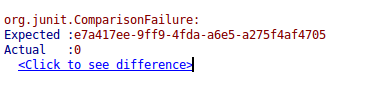
\includegraphics[width=1\textwidth]{./Images/Error_Consumer-GET}
    \caption{Fehlgeschlagenes Assert aufgrund der falschen DataID}
    \label{fig:ErrorConsumerGet}
\end{figure}

Bei get a Metadata Entry den Rückgabewert von getDataId manuell auf String 0 angepasst, Assert schlägt fehl. Weitere Daten können nur überprüft werden, wenn man die Testdaten kennt. Header und ähnliches übernimmt Spring mit dem RestTemplate

Bei einem weiteren Testfall auf der Seite des Consumers wurde mit Absicht eine Eigenschaft des Headers im Request falsch gesetzt. Diese Art von Fehler kann auftreten, wenn bei der Implementierung des Aufrufes der Header falsch gesetzt wird, aber bei der Implementierung des PACT-Fragments korrekt. Beim POST-Aufruf soll der Content-Type "application/json" sein. Dies ist auch so im PACT-Fragment definiert. Hier wurde jedoch der Aufruf angepasst, so dass der Content-Type auf "text/plain" festgelegt wurde. In der Konsole erschien darauf die in \ref{lst:ErrorHeaderConsumer} auf \pageref{lst:ErrorHeaderConsumer} dargestellte Meldung, wobei der Stacktrace gekürzt wurde.

\begin{lstlisting}[caption=Fehler im Header,label={lst:ErrorHeaderConsumer}]
org.springframework.web.client.HttpServerErrorException: 500 Internal Server Error
..

au.com.dius.pact.consumer.PactMismatchException: Pact verification failed for the following reasons:
createMetadata:
    HeaderMismatch - Expected header 'Content-Type' to have value 'application/json' but was 'text/plain'
    BodyTypeMismatch(application/json,text/plain)

The following requests were not received:
Interaction: createMetadata
	in state None
request:
	method: POST
	path: /metadata
	query: null
	headers: [Content-Type:application/json]
	matchers: 
	[$.body.projectId:[match:integer], $.body.userId:[match:integer]]
	body: au.com.dius.pact.model.OptionalBody(PRESENT, 
	{"description":"Test Metadate created via PACT","privacy":"PRIVATE",
	"title":"Test Metadata PACT","type":"GIS","projectId":1,"userId":1})

response:
	status: 201 
	headers: [Content-Type:text/plain] 
	matchers: [$.body:
	[regex:[0-9a-f]{8}-[0-9a-f]{4}-[0-9a-f]{4}-[0-9a-f]{4}-[0-9a-f]{12}]] 
	body: au.com.dius.pact.model
	.OptionalBody(PRESENT, ba501910-5b3c-4bae-ac68-a56bafc793f2)
\end{lstlisting}

Für das Testen des Provider wurden mehrere verschiedene Testfälle erstellt. Beim ersten Test sollte der Provider einen fehlerhaften Body zurückgeben. Dafür wurde die GET-Interaktion verwendet, welche einen spezifischen Metadata-Eintrag zurück gibt. Da zum Zeitpunkt des Testens der Geoserver, welcher bei der Erstellung von Metadata-Einträgen aufgerufen wird,  ausgefallen war, waren alle erstellten Testdaten defekt. Dies kam bei diesem Testfall sehr entgegen, da keine Daten manuell manipuliert werden mussten. Der Testfall ist dahingehend besonders interessant, dass dies wahrscheinlich ein seh häufiger Fehler ist, der beim Schnittstellen Test auftaucht. Selbst kleine Änderung an der Schnittstelle oder an dem Objekt, welches angefragt wird, kann dazu führen, dass das angefragte Objekt bei der Antwort anders aussieht. 
Durch den Ausfall des Geoservers enthielten alle Metadata-Einträge keine Geo-Informationen, welcher in der MAP "additionalTypeSpecificData" gespeichert werden. Diese Map fehlte also alle Metadata-Einträgen. Dieses Fehlen produzierte die auf Seite \pageref{lst:ErrorProvider_GET} dargestellte \ref{lst:ErrorProvider_GET} Fehlermeldung.

\lstset{language = Java}
\begin{lstlisting}[caption=Test,label={lst:ErrorProvider_GET}]
Verifying a pact between metadata-client and metadata-service
  [Using file /home/alex/Mars/mars-import/metadata-client/
  target/pacts/metadata-client-metadata-service.json]
  Get a metadata entry
    returns a response which
      has status code 200 (OK)
      includes headers
        "Content-Type" with value "application/json; charset=UTF-8" (OK)
      has a matching body (FAILED)

Failures:

0) Verifying a pact between metadata-client and metadata-service - 
Get a metadata entry returns a response which has a matching body
      $.body.additionalTypeSpecificData -> Type mismatch: 
      Expected Map Map(bottomRightBound -> 
      Map(lat -> 1954648900, lng -> 1613291745), 
      topLeftBound -> Map(lat -> 4134225878, lng -> 3873370324)) 
      but received Null null

      Diff:

      @1
      -    "additionalTypeSpecificData": {
      -        "bottomRightBound": {
      -            "lat": 1954648900,
      -            "lng": 1613291745
      -        },
      -        "topLeftBound": {
      -            "lat": 4134225878,
      -            "lng": 3873370324
      -        }
      -    },
      +    "additionalTypeSpecificData": null,
          "dataId": "86fc448c-7cac-48cf-88e1-e3bbdfc2452e",
      
      @12
          "dataId": "86fc448c-7cac-48cf-88e1-e3bbdfc2452e",
      -    "description": "CdWPkGgzoyOIPJJbjZah",
      +    "description": "GIS Import via Postman",
          "errorMessage": null,
      
      @16
          "privacy": "PRIVATE",
      -    "projectId": 376674471,
      +    "projectId": 1,
          "records": null,
      
      @19
          "state": "UPLOADED",
      -    "title": "NPQsfuCfIeUsNkKmnczm",
      +    "tags": null,
      +    "title": "Postman Import",
          "type": "GIS",
      
      @21
          "type": "GIS",
      -    "userId": 994762534
      +    "userId": 1
      }
\end{lstlisting}

Im nächsten Testfall für den Provider wurde wieder der Header manipuliert, aber dieses mal jedoch auf der Seite des Response. Für diesen Testfall wurde die PUT-Interaktionenausgewählt, die den Wert aktualisiert, welcher den aktuellen Zustand des Uploads beschreibt. Dafür wurde der Fehler im PACT-Fragment gesetzt und nicht der Metadata-Service angepasst, da dies deutlich aufwendiger gewesen wäre. Für den Response-Header wurde die Eigentschaft auf "Content-Length" auf "1" gesetzt, da der Response Body auf die PUT-Abfrage leer ist, ist die Content-Length auch null. Dies führte zu der auf Seite \pageref{lst:ErrorProvider_PUT} in Listing \ref{lst:ErrorProvider_PUT} aufgeführten Meldung.

\begin{lstlisting}[caption=Test,label={lst:ErrorProvider_PUT}]
Verifying a pact between metadata-client and metadata-service
  [Using file /home/alex/Mars/mars-import/metadata-client/target/pacts/metadata-client-metadata-service.json]
  Set a new state for a metadata entry
    returns a response which
      has status code 200 (OK)
      includes headers
        "Content-Length" with value "1" (FAILED)
      has a matching body (OK)

Failures:

0) Verifying a pact between metadata-client and metadata-service - Set a new state for a metadata entry returns a response which Verifying a pact between metadata-client and metadata-service
  [Using file /home/alex/Mars/mars-import/metadata-client/target/pacts/metadata-client-metadata-service.json]
  Set a new state for a metadata entry
    returns a response which
      has status code 200 (OK)
      includes headers
        "Content-Length" with value "1" (FAILED)
      has a matching body (OK)

Failures:

0) Verifying a pact between metadata-client and metadata-service - Set a new state for a metadata entry returns a response which includes headers "Content-Length" with value "1"
      Expected header 'Content-Length' to have value '1' but was '0'
\end{lstlisting}
      
Beim nächsten Testfall sollte der Statuscode nicht mit dem vorher definierten Statuscode übereinstimmen. Dieser Fehler kann schnell auf der Seite des Providers auftauchen, wenn der Provider mit der Anfrage nicht umgehen kann oder einfach aufgrund von "Coyp and Paste" ein falscher Statuscode für die Rückgabe definiert wurde. Der Testfall konnte leicht umgesetzt werden, indem mit der DELETE-Interaktion ein Metadata-Eintrag gelöscht werden sollte, welcher gar nicht vorhanden ist. Daher gibt der Provider den Statuscode 404 zurück und nicht wie im PACT-Fragment definiert 200. Dadurch kommt die in Listing \ref{lst:ErrorProvider_DELETE} auf Seite \pageref{lst:ErrorProvider_DELETE} abgebildete Meldung.  

\begin{lstlisting}[caption=Test,label={lst:ErrorProvider_DELETE}]
Verifying a pact between metadata-client and metadata-service
  [Using file /home/alex/Mars/mars-import/metadata-client/target/pacts/metadata-client-metadata-service.json]
  Delete a metadata entry
    returns a response which
      has status code 200 (FAILED)
      has a matching body (OK)

Failures:

0) Verifying a pact between metadata-client and metadata-service - Delete a metadata entry returns a response which has status code 200
      assert expectedStatus == actualStatus
             |              |  |
             200            |  404
                            false
\end{lstlisting}

Der letzte Testfall war in dem Sinne gar nicht vorgesehen wie die anderen beschriebenen Testfälle. Beim Erstellen eines neuen Metadata-Eintrags mithilfe der POST-Interaktion, soll eine DataID, welche im UUID-Format vorliegen soll, als einfacher Text zurück gegeben werden. Dafür wurde auch im PACT-Fragment definiert, dass die Antwort eine UUID ist und der Content-Type "plain/text" ist. Die DataID wird für jeden neuen Metadata-Eintrag neu erstellt und der Wert wird zufällig bestimmt. Deswegen ist im PACT-Fragment die Übeprüfung für den Response Body so definiert wurden, dass keine exkate Überprüfung des Wertes stattfindet, sondern eine Überprüfung über reguläre Ausdrücke.  Mit der Überprüfung via reguläre Ausdrücke wird nur getestet, ob der zurück gegebene Wert im UUID-Format vorliegt. Obwohl das Fragment so für diese Überprüfung so erstellt wurde, wie es in der PACT Dokumentation beschrieben wurden ist, erschien die auf Seite \pageref{lst:ErrorProvider_POST} in Listing \ref{lst:ErrorProvider_POST} abgebildete Fehlermeldung. Wie man der Meldung entnehmen kann, schlug die Überprüfung fehl, da die DataIDs unterschiedlich ist. In der Dokumentation gab es keine weitergehende Informationen zu diesem Verhalten.

\begin{lstlisting}[caption=Test,label={lst:ErrorProvider_POST}]
Verifying a pact between metadata-client and metadata-service
  [Using file /home/alex/Mars/mars-import/metadata-client/target/pacts/metadata-client-metadata-service.json]
  createMetadata
    returns a response which
      has status code 201 (OK)
      includes headers
        "Content-Type" with value "text/plain" (OK)
      has a matching body (FAILED)

Failures:

0) Verifying a pact between metadata-client and metadata-service - createMetadata returns a response which has a matching body
      / -> mismatch

      Diff:

      @0
      -d08f46fd-95e9-432c-95c2-7b1a0a078162
      +326e27d7-6285-45de-8343-36b3ab3798f8
\end{lstlisting}

Damit sind alle Testfalle beschrieben wurden, welche ausgeführten wurden, um PACT bewerten zu können.

\subsection{Bewertung der Ergebnisse}
Das Fazit und die damit verbundene Bewertung für PACT soll in zwei grobe Bereiche unterteilt werden. Einmal die Einbindung von PACT in ein bestehendes System und zum anderen die Bewertung der ausgeführten Testfälle.

Im Gegensatz zu dem am Anfang beschriebenen Ansatz, bei dem PACT bei der Implementierung des Consumers mit eingebunden wird, musste bei MARS PACT in ein bestehendes System eingebunden werden. Ergänzend dazu kam, dass man selber weder den Metadata-Client noch den Metadata-Service implementiert hatte. Im generellen Ablauf von PACT wird jedoch davon ausgegangen, dass man Consumer sowie den Provider selber implmentiert. Dieser Umstand führte zu einigen Schwierigkeiten.
Denn es waren nicht immer alle notwendigen Informationen vorhanden. Zwar lieferten die Swagger-Dateien sehr wichtige Informationen, jedoch waren diese nicht immer korrekt oder waren veraltet. Zudem fehlten auch einige Informationen. Auch wenn man diese Informationen teilweise über die Analyse der Aufrufe via Chrome herausarbeiten konnte, war dies jedoch mit deutlichem mehraufwand verbunden. Dieser Mehraufwand wäre vermutlich nict vorhanden, wenn man das System genau kennen würde.

Aufgrund der fehlenden Informationen konnte man auch nicht immer entscheiden, ob das aktuelle Verhalten korrekt ist. Deswegen gab es teilweise auch keine andere Möglichkeit als das aktuelle Verhalten als das Soll-Verhalten zu definieren, um sich auch nicht selber aufzuhalten. Zudem konnte wegen den fehlenden Inoformationen keine Priosierung vorgenommen werden. Es war nicht klar, welche Aspekte unbedingt getestet werden müssen und welche nicht. Ein einfaches Beispiel dafür kann man nennen, dass man teilweise nicht wusste, ob eine bestimmte Eigenschaft des Headers getestet werden muss.

Um die einzelnen Interaktionen besser zu verstehen, war es unumgänglich die Interaktion zuerst in Postman umzusetzen. Denn damit bekamm eine bessere Übersicht wie genau die Anfragen auszusehen haben und wie die Antworten aufgebaut sind. Erst mit diesen Informationen konnten die Implementierung von PACT beginnen.

Jedoch war die Implementierung von PACT auch nicht ganz ohne Schwierigkeiten. Schaut man sich zuerst beschriebene generelle Beispiel und die danch erfolgte Implementierung in MARS an, sieht es auf den ersten Blick sehr kopmakt und vor allem simpel aus. Im Prinzip ist es auch simpel und kompakt, wenn man es verstanden hat. Jedoch ist leider die Dokumentation von PACT ausbaufähig. Dies erschwerte den Aufbau des Verständnis.

In der PACT Dokumentation werden viele Aspekte nur kurz erläutert. Teilweise werden Aspekte nur mithilfe eines Beipieles ohne aussagekräftige Beschreibung dargestellt. Problematisch wurde es dann, wenn die gezeigten Beispiele nicht für den aktuelle Situation übertrag waren. Dann war man auf die teilweise sehr kurze Erklärung angewiesen. Dies führte manchmal dazu, dass man einige Abschnitte mit der Methode "try and error" implementierte, also so lange ausprobierte, bis es funktionierte. Besonders die erste Erstellung eines JSON-Body mit PACT war sehr aufwendig, bis man verstanden hatte, was die einzelnen Methoden genau machten. Erschwerend kam hinzu, dass es mehrere Beschreibungen für die gleiche Abschnitte gab, die jedoch für verschiedene Versionen gültig waren. Dadurch wurde es manchmal sehr unübersichtlich, da man immer wieder prüfen musste, ob die Erklärung für die verwendete Version passt.

Zu der ausbaufähigen Dokumentation kam leider noch hinzu, dass PACT noch nicht sehr verbreitet ist. Wegen der Dokumentation war man immer wieder in der Situation bestimmte Sachverhalte bzw. Fragestellungen im Internet zu suchen. Das Ergebnis war leider sehr oft entäuschend. Wenn überhaupt gab es nur eine kurze Beschreibung in Form eines Git-Issues. Wobei diese meistens Fehler aus voherigen Versionen beschrieben, die in der verwendeten Version schon behoben waren. Daher konnten nicht immer Antworten gefunden werden und man verließ sich wieder auf "try and error".

Zusammenfassend für den Abschnitt der Einbindung von PACT in MARS kann man jedoch sagen, dass es durchaus simpel und schnell umsetzbar ist. Dies setzt aber voraus, dass man sowohl weiß, wie der Consumer und Provider im Deatil interagieren und wie man mit PACT die Testfälle implementiert.

Im nächsten bereich werden die einzelnen Untersuchungen bewertet. Zum Beginn kann man gleich festhalten, dass die Ausführung der Tests, egal ob es auf der Seite des Consumers oder Providers ist, sehr schnell ausgeführt werden. Dadurch bekommt man sehr schnell ein Feedback, ob die Tests erfolgreich waren. 

Wie man gut aus manchen Listings ableiten kann, sind die Meldungen teilweise sehr lang. Besonders bei einigen Fehlern wiederholen sich die Fehlerbeschreibungen und sorgen für eine lange Meldung in der Konsole. Unter anderem dadurch werden die Meldung unübersichtlich und man muss genau lesen, woran der Test gescheitert ist. Besonders bei der Meldung, die in \ref{lst:ErrorProvider_GET} auf Seite \pageref{lst:ErrorProvider_GET}, ist die Fehler Beschreibung verwirrend und teilweise auch einfach falsch. Wie die Fehlerbeschreibung korrekt wiedergibt, fehlt einfach die Map mit den GEO-Daten. Jedoch werden im Diff-Abschnitt auch andere Body-Abschnitte angezeigt, die sich unterscheiden. Dabei ist für diese Abschnitte definiert wurden, dass nur der Typ bzw. Format geprüft werden soll und keine Überprüfung des Wertes. Die komplette Meldung suggeriert aber, dass auch diese Abschnitte fehlerhaft sind. Dies führte durchaus zu Verwirrungen und lenkte von der eigentlichen Unterscheidung ab. 
 
Auch die im Listing \ref{lst:ErrorHeaderConsumer} auf Seite \pageref{lst:ErrorHeaderConsumer} abgebildete Meldung ist unübersichtlich. Zwar gibt die Fehlermeldung, dass ein der Wert von der Eigenschaft \enquote{Accept} im Header nicht stimmt, exakt wieder. Jedoch gibt es keinen Verweis darauf, dass es sich um den Request-Header handelt. Dazu wird nur angegeben, welcher Request nicht empfangen wurde. Eine Ansicht, in der die Unterschiede gegenüber gestellt werden, wäre sinnvoller.
Das Ähnliche gilt auch für das Listing \ref{lst:ErrorProvider_PUT} auf Seite \pageref{lst:ErrorProvider_PUT}. Die Fehlermeldung wird eindeutig beschrieben. Jedoch ist auch hier die Ausgabe sehr umfangreich und wiederholt sich zum Teil auch einfach. Besonders die Länge der Meldungen und den teilweise unnötigen Anzeigen von Unterschieden macht die Rückmeldungen von PACT sehr unübersichtlich. Dies trifft verstärkt auf, wenn die Tests nicht einzelnd ausgeführt werden, sondern zusammen. Sollten dann mehrere Tests fehlschlagen, kann die Meldung sehr lang werden und damit auch sehr  unübersichtlich. Was dazu führen kann, dass Fehler zunächst übersehen werden oder falsch interprtiert werden.

Als gutes Beispeil für eine gelungene Fehler Ausgabe, kann man das Listing \ref{lst:ErrorProvider_DELETE} auf Seite \pageref{lst:ErrorProvider_DELETE} nehmen. Es ist kurz und knapp beschrieben, wo der Fehler liegt. Daher ist es klar erkennbar, dass der Statuscode in der Response nicht stimmt. Zudem ist die Gegenüberstellung der Statuscodes sehr hilfreich.

Eine Berwetung der Ausgabe bei erfolgreichen Tests wird hier nicht speziell betrachtet, da nur die Meldung erscheint, dass die Tests erfolgreich waren. Dies betrifft sowohl die Tests auf Seite des Consumers sowie auf der Seite des Providers.

Ein weiterer negativer Punkt ist die in Listing \ref{lst:ErrorProvider_POST} auf Seite \pageref{lst:ErrorProvider_POST} abgebildete Meldung. Der Test sollte erfolgreich sein, da nur überprüft werden soll, ob der String im Body der Reponse im Format einer UUID vorliegt. Der zurückgebene String liegt auch im UUID-Format vor. Daher scheint dies ein Fehler in PACT zu sein. 

Abschließend kann man über PACT sagen, dass sich die Verwendung von PACT durchaus lohnt. Der Vorteil, des schnellen Feedbacks und der durchaus schnellen Implementierung der Tests, überweiegt die Nachteile zu den teilweise uneindeutigen und/oder zu langen Fehlermeldung. Auch der zuletzt beschriebene Fehler ändert daran nichts. Mit PACT bekommen die Entwickler eine schnelle Rückmeldung, ob ihre Änderugen zu ungewollten Veränderungen der Schnittstellen führen oder sie können schnell überblicken bei gewollten Veränderungen der Schnittstellen, welche Anpassungen sie vornehmen müssen.

Eine Vorraussetzung für die Verwendung von PACT sollte jedoch sein, dass sie ähnlich wie Unit-Tests bei den Entwicklern angesiedelt werden sollten. Das heißt die Implementierung sollten von den Entwicklern vorgenommen werden, welche auch die Consumer und Provider entwickeln. Es ist sehr hilfreich bei der Implementierung von PACT zu wissen, was genau getestet werden soll und wo die Schwerpunkte liegen. Als Beispiel kann man dafür die Header nehmen. Als Außenstehender ist es schwer zu wissen, ob Eigenschaften überprüft werden sollen und wenn ja, welche genau. Diese Entscheidungen können die Entwickler besser treffen, da sie die Testobjekte detailierter kennen. Als ALternative ginge auch, dass die Entwickler genau spezifieren, was getestet werden soll und eine dritte Person, die Implementierung von PACT übernimmt. Dabei muss aber die Spezifierung sehr genau sein, damit die Person, die PACT implementiert, auch genau weiß, was getestet werden muss und wo die Schwerpunkte liegen. 

PACT ist durchaus geeignet für MARS bzw. für Microservice Architekturen. Jedoch müssen die oben genannten Vorraussetzungen stimmen. Zwar ist die Implementierung in ein bestehendes System umfangreicher als, wenn man PACT von Anfang mit implemtiert. Jedoch sind die Vorteile, wie das schnelle Feedback, sehr sinnvoll für ein System, das sich ständig ändert. Denn mit PACT kann man sehr gut prüfen, ob Änderungen zu ungewollten Änderungen der Schnittstelle führen oder welche Services noch aktualisiert werden müssen.

\section{Ausblick Masterarbeit}
In der Master Arbeit sollen die begonnen Arbeiten aus den bisherigen Projekten und den Seminaren fortgesetzt werden. Ein Schwerpunkt wird dabei die Im Hauptseminar begonne Ausarbeitung zu dem Testkonzept von Google und das von Martin Fowler erstellte Testkonzept für Programme, die eine Microserservice-Architektur verwenden. Ergänzend zu diesen beiden Konzepte sollen weitere aktuelle Testkonzepte gesammelt und verglichen werden. Interessant dabei sein wird herauszufinden, wie andere große Software Hersteller wie z.B. Microsoft, zurzeit ihre Software testen. Dies wird unter der Fragestellung stehen: Mit welchem Konzepten wird Software heutzutage getestet?

Diese Konzepte sollen nicht auschließlich untereinander verglichen werden, sondern auch mit bisherigen Testkonzepten verglichen werden. Dabei soll heraus gearbeitet werden, wie sich die Testkonzepte entwickelt haben und ob es einen allgemein gültigen Trend gibt. Dazu sollen die Testkonzepte noch unter dem Aspekt untersucht werden, wie gut sie sich für eine Microserive Architektur eignen könnten.

Ein weiterer Schwerpunkt soll auf der Automatisierung der Testfall-Erstellung liegen. Mit dem Programm Postman ist es schon möglich mithilfe einer Schnittstellen-Beschreibung wie z.B. mit einer Swagger-Datei automatisch Konstrukte für Testfälle zu erstellen. Jedoch müssen die Tests noch mit Daten gefüllt werden. Dazu erstellt Postman nur einen Testfall pro Interaktion. Jedoch wären mehrere Testfälle pro Interaktion sinnvoller, um verschiedene Möglichkeiten und Pfade abzudecken. Zudem fehlt den Testfällen ein definiertes Soll-Ergebnis gegen das geprüft werden kann. 

Wegen den eben geannten Defiziten ist es interessant zu forschen, inwieweit man diese Defizite beheben kann. Eine mögliche Lösung könnte sein die Beschreibung der Schnittstelle so zu erweiteren, dass fehlende Informationen wie Testdaten und Soll-Ergebnis mit abgebildet werden. In diesem Zusammenhang stellt sich auch die Frage, ob eine Modell-Beschreibung der Schnittstelle sinnvoller wäre und ob sogar die Beschreibung der Schnittstelle in der Swagger-Datei nicht schon eine Modell-Beschreibung ist. Für den gesamten Aspekt der Automatisierung der Testfall Erstellung können etablierte Konzepte wie das Model-Based Testing sehr nützlich sein. Model-Based Testing beruht darauf auf der Grundlage von Modellen Testfälle zu erstellen und durchzuführen. Deswegen ist es sinnig, wenn man sich mit der automatischen Testfall Erstellung auseinander setzt, sich in diesem Zuge auch mit Model-Based Testing auseinander zu setzen. Denn Model-Based Testing ist ein etlabiertes Konzept, was für viele Probleme, die in diesem Zusammenhang auftauchen können, Lösungen gefunden hat. Diese Lösungen können ggf. wieder verwendet werden oder angepasst verwendet werden. 

\bibliography{literatur}
\bibliographystyle{alpha}

\end{document}